\emph{seasonal} is an easy-to-use and full-featured R-interface to
X-13ARIMA-SEATS, the newest seasonal adjustment software developed by
the \href{http://www.census.gov/srd/www/x13as/}{United States Census
Bureau}. X-13ARIMA-SEATS combines and extends the capabilities of the
older X-12ARIMA (developed by the Census Bureau) and TRAMO-SEATS
(developed by the Bank of Spain).

\begin{figure}[htbp]
\centering
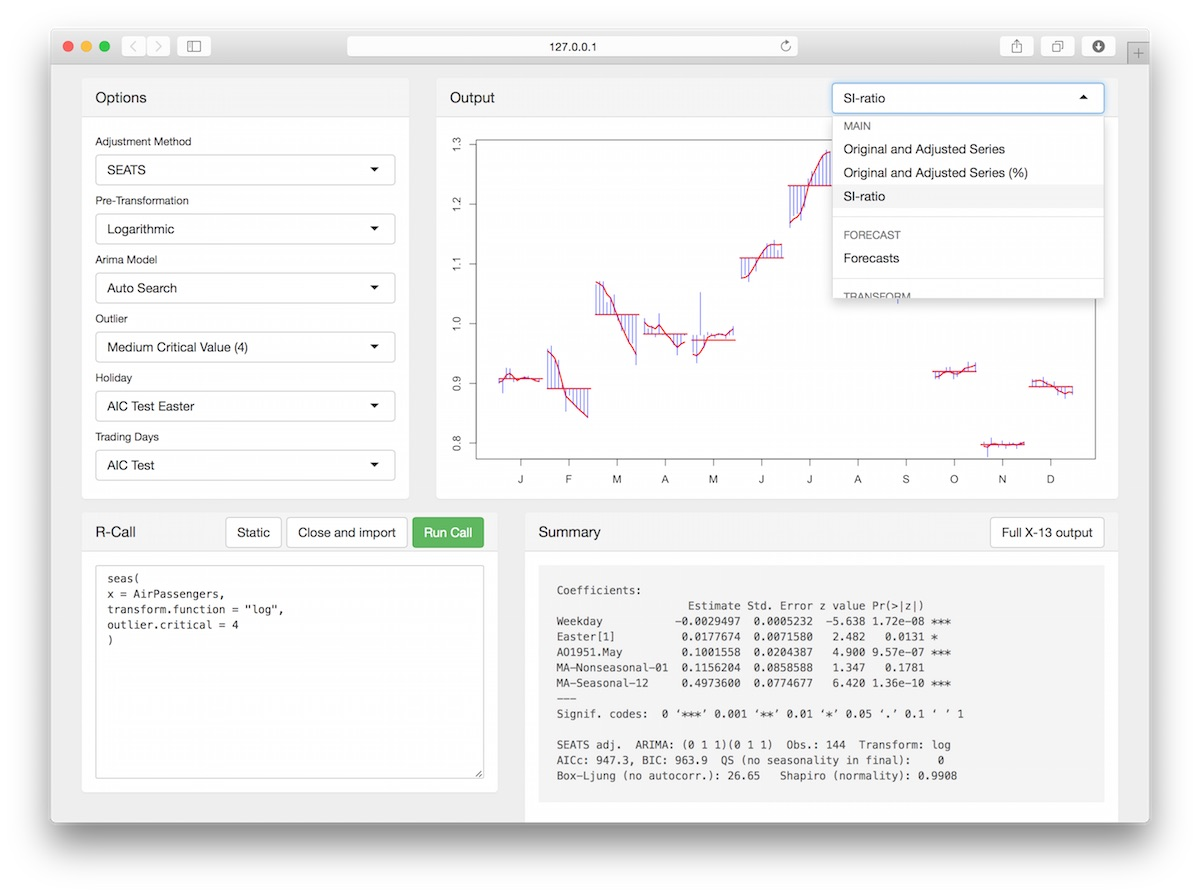
\includegraphics[width=\textwidth]{images/inspect.jpg}
\caption{Graphical user interface for X-13}
\end{figure}

If you are new to seasonal adjustment or X-13ARIMA-SEATS, the automated
procedures of \emph{seasonal} allow you to quickly produce good seasonal
adjustments of time series. Start with the
\hyperref[installation]{Installation} and
\hyperref[getting-started]{Getting started} section and skip the rest.
Alternatively, \texttt{demo(seas)} gives an overview of the package
functionality.

If you are familiar with X-13ARIMA-SEATS, you may benefit from the
flexible input and output structure of \emph{seasonal}. The package
allows you to use (almost) all commands of X-13ARIMA-SEATS, and it can
import (almost) all output generated by X-13ARIMA-SEATS. The only
exception is the `composite' spec, which is easy to replicate in basic
R. Read the \hyperref[input]{Input} and \hyperref[output]{Output}
sections and have a look at the
\href{https://github.com/christophsax/seasonal/wiki/Examples-of-X-13ARIMA-SEATS-in-R}{wiki},
where the examples from the official X-13ARIMA-SEATS
\href{http://www.census.gov/ts/x13as/docX13ASHTML.pdf}{manual} are
reproduced in R.

\hyperdef{}{installation}{\section{Installation}\label{installation}}

\subsection{Getting seasonal}\label{getting-seasonal}

The stable version is available from CRAN:

\begin{verbatim}
install.packages("seasonal")
\end{verbatim}

To install the latest development version directly from Github, type to
the R console:

\begin{verbatim}
install.packages("devtools")       
devtools::install_github('christophsax/seasonal')      
\end{verbatim}

\subsection{Getting X-13}\label{getting-x-13}

\emph{seasonal} does not include the binary executables of
X-13ARIMA-SEATS. They can be obtained precompiled from
\href{http://www.census.gov/srd/www/x13as/x13down_pc.html}{here}
(Windows: \texttt{x13ashtmlall.zip}). There are guides for building it
from source for
\href{http://askubuntu.com/questions/444354/how-do-i-install-x13-arima-seats-for-rstudio-from-source}{Ubuntu}
or
\href{https://github.com/christophsax/seasonal/wiki/Compiling-X-13ARIMA-SEATS-from-Source-for-OS-X}{Mac
OS-X}.

Download the file, unzip it and copy \texttt{x13ashtml.exe} (or
\texttt{x13ashtml}, on a Unix system) to any desired location on your
file system.

\subsection{Telling R where to find
X-13}\label{telling-r-where-to-find-x-13}

Next, you need to tell \emph{seasonal} where to find the binary
executables of X-13ARIMA-SEATS, by setting the specific environmental
variable \texttt{X13\_PATH}. This may be done during your active session
in R:

\begin{verbatim}
Sys.setenv(X13_PATH = "YOUR_X13_DIRECTORY")
\end{verbatim}

Exchange \texttt{YOUR\_X13\_DIRECTORY} with the path to your
installation of X-13ARIMA-SEATS. Note that the Windows path
\texttt{C:\textbackslash{}something\textbackslash{}somemore} has to be
entered UNIX-like \texttt{C:/something/somemore} or
\texttt{C:\textbackslash{}\textbackslash{}something\textbackslash{}\textbackslash{}somemore}.
You can always check your installation with:

\begin{verbatim}
checkX13()
\end{verbatim}

If it works, you may want to set the environmental variable permanently,
by adding the \texttt{Sys.setenv} line to one of your \texttt{.Rprofile}
files. The easiest is to use the one located in your home directory,
which can be written directly from R:

\begin{verbatim}
write('Sys.setenv(X13_PATH = "YOUR_X13_DIRECTORY")', 
      file = "~/.Rprofile", append = TRUE)
\end{verbatim}

If the file does not exist (by default), it will be created. Make sure
that you get the quotes right: double quotes around your directory,
single quotes around the whole \texttt{Sys.setenv} line, such that R
understands your string. Check first that the the \texttt{Sys.setenv}
line works correctly; once it is written you may have to edit
\texttt{.Rprofile} manually. (Or add a second, overwriting line to it.)
For other ways to set an environmental variable permanently in R, see
\texttt{?Startup}.

\hyperdef{}{getting-started}{\section{Getting
started}\label{getting-started}}

seas is the core function of the \emph{seasonal} package. By default,
seas calls the automatic procedures of X-13ARIMA-SEATS to perform a
seasonal adjustment that works well in most circumstances:

\begin{verbatim}
m <- seas(AirPassengers)
 
\end{verbatim}

The first argument of \texttt{seas} has to be a time series of class
\texttt{"ts"}. The function returns an object of class \texttt{"seas"}
that contains all necessary information on the adjustment.

There are several functions and methods for \texttt{"seas"} objects: The
\texttt{final} function returns the adjusted series, the \texttt{plot}
method shows a plot with the unadjusted and the adjusted series. The
\texttt{summary} method allows you to display an overview of the model:

\begin{verbatim}
final(m)
plot(m)
summary(m)
\end{verbatim}

By default, \texttt{seas} calls the SEATS adjustment procedure. If you
prefer the X11 adjustment procedure, use the following option (see the
\hyperref[input]{Input} section for details on how to use arbitrary
options with X-13):

\begin{verbatim}
seas(AirPassengers, x11 = "")
\end{verbatim}

A default call to \texttt{seas} also invokes the following automatic
procedures of X -13ARIMA-SEATS:

\begin{itemize}
\itemsep1pt\parskip0pt\parsep0pt
\item
  Transformation selection (log / no log)
\item
  Detection of trading day and Easter effects
\item
  Outlier detection
\item
  ARIMA model search
\end{itemize}

Alternatively, all inputs may be entered manually, as in the following
example:

\begin{verbatim}
seas(x = AirPassengers, 
     regression.variables = c("td1coef", "easter[1]", "ao1951.May"), 
     arima.model = "(0 1 1)(0 1 1)", 
     regression.aictest = NULL,
     outlier = NULL, 
     transform.function = "log")
\end{verbatim}

The \texttt{static} command returns the manual call of a model. The call
above can be easily generated from the automatic model:

\begin{verbatim}
static(m)
static(m, coef = TRUE)  # also fixes the coefficients
\end{verbatim}

If you have \emph{Shiny} installed, the \texttt{inspect} command offers
an easy way to analyze and modify a seasonal adjustment procedure (see
the section below for details):

\begin{verbatim}
inspect(m)
\end{verbatim}

\hyperdef{}{input}{\section{Input}\label{input}}

In \emph{seasonal}, it is possible to use almost the complete syntax of
X-13ARIMA- SEATS. This is done via the \texttt{...} argument in the
\texttt{seas} function. The X -13ARIMA-SEATS syntax uses \emph{specs}
and \emph{arguments}, with each spec optionally containing some
arguments. These spec-argument combinations can be added to
\texttt{seas} by separating the spec and the argument by a dot
(\texttt{.}). For example, in order to set the `variables' argument of
the `regression' spec equal to \texttt{td} and \texttt{ao1999.jan}, the
input to \texttt{seas} looks like this:

\begin{verbatim}
m <- seas(AirPassengers, regression.variables = c("td", "ao1955.jan"))
\end{verbatim}

Note that R vectors may be used as an input. If a spec is added without
any arguments, the spec should be set equal to an empty string (or,
alternatively, to an empty list, as in previous versions). Several
defaults of \texttt{seas} are empty strings, such as the default
\texttt{seats = ""}. See the help page (\texttt{?seas}) for more details
on the defaults. Note the difference between \texttt{""} (meaning the
spec is enabled but has no arguments) and \texttt{NULL} (meaning the
spec is disabled).

It is possible to manipulate almost all inputs to X-13ARIMA-SEATS in
this way. The best way to learn about the relationship between the
syntax of X-13ARIMA-SEATS and \emph{seasonal} is to study the
\href{https://github.com/christophsax/seasonal/wiki/Examples-of-X-13ARIMA-SEATS-in-R}{comprehensive
list of examples in the wiki}. For instance, example 1 in section 7.1
from the \href{http://www.census.gov/ts/x13as/docX13ASHTML.pdf}{manual},

\begin{verbatim}
series { title  =  "Quarterly Grape Harvest" start = 1950.1
       period =  4
       data  = (8997 9401 ... 11346) }
arima { model = (0 1 1) }
estimate { }
\end{verbatim}

translates to R in the following way:

\begin{verbatim}
seas(AirPassengers,
     x11 = ""),
     arima.model = "(0 1 1)"
)
\end{verbatim}

\texttt{seas} takes care of the `series' spec, and no input beside the
time series has to be provided. As \texttt{seas} uses the SEATS
procedure by default, the use of X11 has to be specified manually. When
the `x11' spec is added as an input (like above), the mutually exclusive
and default `seats' spec is automatically disabled. With
\texttt{arima.model}, an additional spec-argument is added to the input
of X-13ARIMA-SEATS. As the spec cannot be used in the same call as the
`automdl' spec, the latter is automatically disabled.

There are some mutually exclusive specs in X-13ARIMA-SEATS. If more than
one mutually exclusive spec is included in \texttt{seas}, specs are
overwritten according the following priority rules:

\begin{itemize}
\itemsep1pt\parskip0pt\parsep0pt
\item
  Model selection

  \begin{enumerate}
  \def\labelenumi{\arabic{enumi}.}
  \itemsep1pt\parskip0pt\parsep0pt
  \item
    \texttt{arima}
  \item
    \texttt{pickmdl}
  \item
    \texttt{automdl} (default)
  \end{enumerate}
\item
  Adjustment procedure

  \begin{enumerate}
  \def\labelenumi{\arabic{enumi}.}
  \itemsep1pt\parskip0pt\parsep0pt
  \item
    \texttt{x11}
  \item
    \texttt{seats} (default)
  \end{enumerate}
\end{itemize}

As an alternative to the \texttt{...} argument, spec-arguments can also
be supplied as a named list. This is useful for programming:

\begin{verbatim}
seas(list = list(x = AirPassengers, x11 = ""))
\end{verbatim}

\hyperdef{}{output}{\section{Output}\label{output}}

\emph{seasonal} has a flexible mechanism to read data from
X-13ARIMA-SEATS. With the \texttt{series} function, it is possible to
import almost all output that can be generated by X-13ARIMA-SEATS. For
example, the following command returns the forecasts of the ARIMA model
as a \texttt{"ts"} time series:

\begin{verbatim}
m <- seas(AirPassengers)
series(m, "forecast.forecasts")
\end{verbatim}

Because the \texttt{forecast.save = "forecasts"} argument has not been
specified in the model call, \texttt{series} re-evaluates the call with
the `forecast' spec enabled. It is also possible to return more than one
output table at the same time:

\begin{verbatim}
series(m, c("forecast.forecasts", "d1"))
\end{verbatim}

You can use either the unique short names of X-13 (such as \texttt{d1}),
or the the long names (such as \texttt{forecasts}). Because the long
table names are not unique, they need to be combined with the spec name
(\texttt{forecast}). See \texttt{?series} for a complete list of
options.

Note that re-evaluation doubles the overall computation time. If you
want to speed it up, you have to be explicit about the output in the
model call:

\begin{verbatim}
m <- seas(AirPassengers, forecast.save = "forecasts")
series(m, "forecast.forecasts")
\end{verbatim}

Some specs, like `slidingspans' and `history', are time consuming.
Re-evaluation allows you to separate these specs from the basic model
call:

\begin{verbatim}
m <- seas(AirPassengers)
series(m, "history.saestimates")
series(m, "slidingspans.sfspans")
\end{verbatim}

If you are using the HTML version of X-13, the \texttt{out} function
shows the content of the main output in the browser:

\begin{verbatim}
out(m)
\end{verbatim}

\section{Graphs}\label{graphs}

There are several graphical tools to analyze a \texttt{seas} model. The
main plot function draws the seasonally adjusted and unadjusted series,
as well as the outliers. Optionally, it also draws the trend of the
seasonal decomposition:

\begin{verbatim}
m <- seas(AirPassengers, regression.aictest = c("td", "easter"))
plot(m)
plot(m, outliers = FALSE)
plot(m, trend = TRUE)
\end{verbatim}

The \texttt{monthplot} function allows for a monthwise plot (or
quarterwise, with the same function name) of the seasonal and the SI
component:

\begin{verbatim}
monthplot(m)
monthplot(m, choice = "irregular")
\end{verbatim}

Also, many standard R function can be used to analyze a \texttt{"seas"}
model:

\begin{verbatim}
pacf(resid(m))
spectrum(diff(resid(m)))
plot(density(resid(m)))
qqnorm(resid(m))
\end{verbatim}

The \texttt{identify} method can be used to select or deselect outliers
by point and click. Click several times to loop through different
outlier types.

\begin{verbatim}
identify(m)
\end{verbatim}

\section{Inspect}\label{inspect}

The \texttt{inspect} function is a graphical tool for choosing a
seasonal adjustment model, using
\emph{\href{http://shiny.rstudio.com}{Shiny}}, with the same structure
as the \href{http://www.seasonal.website}{demo website of seasonal}. To
install the latest version of Shiny, type:

\begin{verbatim}
install.packages("shiny")
\end{verbatim}

The goal of \texttt{inspect} is to summarize all relevant options, plots
and statistics that should be usually considered. \texttt{inspect} uses
a \texttt{"seas"} object as its main argument:

\begin{verbatim}
inspect(m)
\end{verbatim}

Frequently used options can be modified using the drop down selectors in
the upper left panel. Each change will result in a re-estimation of the
seasonal adjustment model. The R-call, the output and the summary are
updated accordingly.

Alternatively, the R-Call can be modified manually in the lower left
panel. Press `Run Call' to re-estimate the model and to adjust the
option selectors, the output, and the summary. With the `Close and
Import' button, inspect is closed and the call is imported to R. The
`static' button substitutes automatic procedures are substituted by the
automatically chosen spec-argument options, in the same way as
\texttt{static}.

The views in the upper right panel can be selected from the drop down
menu. The views can also be customized (see \texttt{?inspect}for
details)

The lower right panel shows the summary, as descibed in the help page of
\texttt{?summary.seas}. The `Full X-13 output' button opens the complete
output of X-13 in a separate tab or window.

\section{Chinese New Year, Indian Diwali and other customized
holidays}\label{chinese-new-year-indian-diwali-and-other-customized-holidays}

seasonal includes \texttt{genhol}, a function that makes it easy to
model user-defined holiday regression effects. \texttt{genhol} is an R
replacement for the equally named software by the Census Office; no
additional installation is required. The function uses an object of
class \texttt{"Date"} as its first argument, which specifies the
occurrence of the holiday.

In order to adjust Indian industrial production for Diwali effects, use,
e.g.,:

\begin{verbatim}
data(seasonal) # Indian industrial production: iip
data(holiday)  # dates of Chinese New Year, Indian Diwali and Easter

seas(iip, 
x11 = "",
xreg = genhol(diwali, start = 0, end = 0, center = "calendar"), 
regression.usertype = "holiday"
)
\end{verbatim}

For more examples, including Chinese New Year and complex pre- and
post-holiday adjustments, see \texttt{?genhol}.

\section{Production use}\label{production-use}

While \emph{seasonal} offers a quick way to adjust a time series in R,
it is equally suited for the recurring processing of potentially large
numbers of time series. There are two kind of seasonal adjustments in
production use:

\begin{enumerate}
\def\labelenumi{\arabic{enumi}.}
\itemsep1pt\parskip0pt\parsep0pt
\item
  a periodic application of an adjustment model to a time series
\item
  an automated adjustment to a large number of time series
\end{enumerate}

This section shows how both tasks can be accomplished with
\emph{seasonal} and basic R.

\subsection{Storing calls and batch
processing}\label{storing-calls-and-batch-processing}

\texttt{seas} calls are R objects of the standard class \texttt{"call"}.
Like any R object, calls can be stored in a list. In order to extract
the call of a \texttt{"seas"} object, you can access the \texttt{\$call}
element or extract the static call with \texttt{static()}. For example,

\begin{verbatim}
# two different models for two different time series
m1 <- seas(fdeaths, x11 = "")
m2 <- seas(mdeaths, x11 = "")

l <- list()
l$c1 <- static(m1)  # static call (with automated procedures substituted)
l$c2 <- m2$call     # original call
\end{verbatim}

The list can be stored and re-evaluated if new data becomes available:

\begin{verbatim}
ll <- lapply(l, eval)
\end{verbatim}

which returns another list containing the re-evaluated \texttt{"seas"}
objects. If you want to extract the final series, use:

\begin{verbatim}
do.call(cbind, lapply(ll, final))
\end{verbatim}

Of course, you also can extract any other series, e.g.:

\begin{verbatim}
# seasonal component of an X11 adjustment, see ?series
do.call(cbind, lapply(ll, series, "d10"))
\end{verbatim}

\subsection{Automated adjustment of multiple
series}\label{automated-adjustment-of-multiple-series}

X-13 can also be applied to a large number of series, using automated
adjustment methods. This can be accomplished with a loop or an apply
function. It is useful to wrap the call to \texttt{seas} in a
\texttt{try} statement; that way, an error will not break the execution.
You need to develop an error handling strategy for these cases: You can
either drop them, use them without adjustment or switch to a different
automated routine.

\begin{verbatim}
# collect data 
dta <- list(fdeaths = fdeaths, mdeaths = mdeaths)

# loop over dta
ll <- lapply(dta, function(e) try(seas(e, x11 = "")))

# list failing models
is.err <- sapply(ll, class) == "try-error"
ll[is.err]

# return final series of successful evaluations
do.call(cbind, lapply(ll[!is.err], final))
\end{verbatim}

If you have several cores and want to speed things up, the process is
well suited for parallelization (thanks, Matthias Bannert):

\begin{verbatim}
# a list with 100 time series
largedta <- rep(list(AirPassengers), 100)

library(parallel)  # R-core team, part of R 

# set up cluster
cl <- makeCluster(detectCores())

# load 'seasonal' for each node
clusterEvalQ(cl, library(seasonal))

# export data to each node
clusterExport(cl, varlist = "largedta")

# run in parallel (2.2s on a 8-core Macbook)
parLapply(cl, largedta, function(e) try(seas(e, x11 = "")))

# compare to standard lapply (9.6s)
lapply(largedta, function(e) try(seas(e, x11 = "")))

# finally, stop the cluster
stopCluster(cl)
\end{verbatim}

\section{License}\label{license}

\emph{seasonal} is free and open source, licensed under GPL-3. It has
been developed for the use at the Swiss State Secretariat of Economic
Affairs and is not related to the development of X-13ARIMA-SEATS
(\href{https://www.census.gov/srd/www/disclaimer.html}{license}).

Please report bugs and suggestions on
\href{https://github.com/christophsax/seasonal}{Github} or send me an
\href{mailto:christoph.sax@gmail.com}{e-mail}. Thank you!
